\section{Introduction}
Recent advances in biomedical image analysis have assisted many pathologists and biologists to facilitate their researches \cite{Chen2016b, Ronneberger2015,Chen2016c,Lieman-Sifry2017,Paszke2016,Tseng2017,Sirinukunwattana2015b}.
Among these researches, a significant application is to obtain the accurate segmentation of specific membrane objects in a biomedical image, such as lumenal glands, synaptic vesicles and cells.
Especially, the morphological shape and spatial distribution of synaptic vesicles are helpful to study the neural activity in different brain regions, while morphological statistics of lumenal glands are widely used for assessment of the malignancy degree of adenocarcinomas.
%
Conventionally, these crucial steps are performed by human expert, which are time-consuming and suffer from subjective factors.
Therefore, it is significantly demanded to improve the efficiency as well as the reliability with automatic segmentation methods.

\begin{figure}
    \begin{center}
        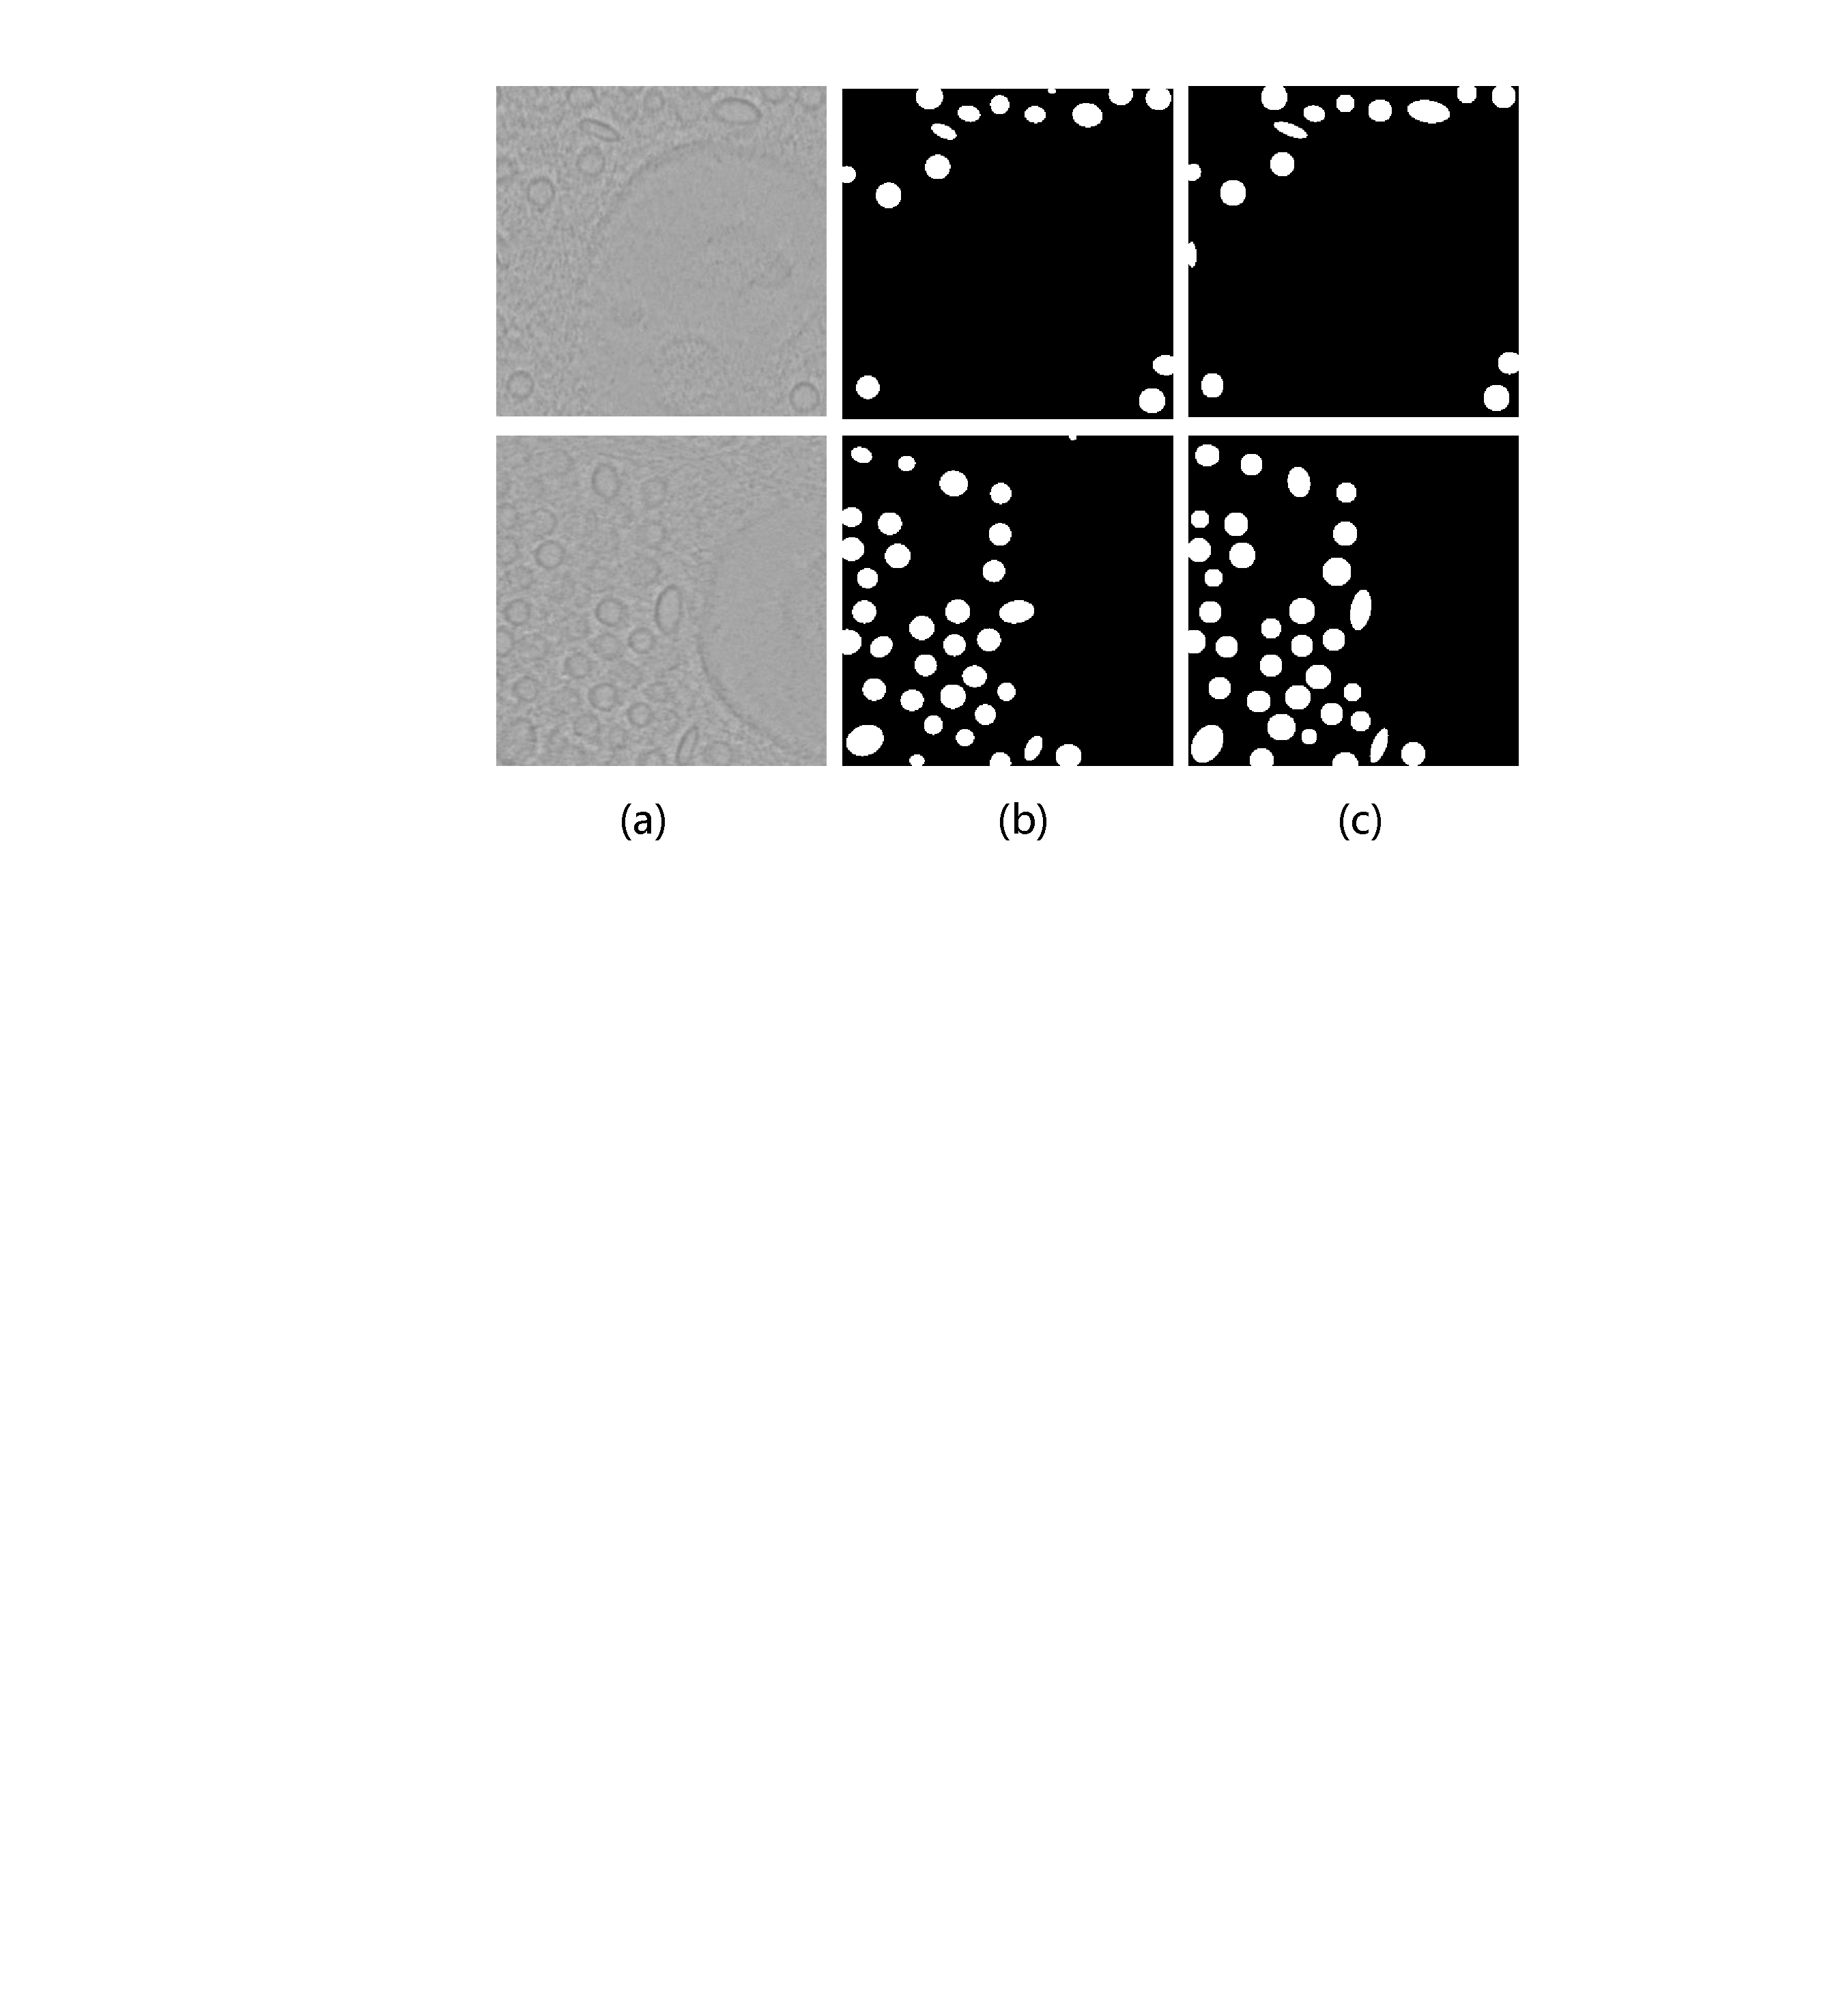
\includegraphics[width=3.3in]{figures/FigImg.pdf}
    \end{center}
    \caption{An example showing the challenges of biomedical segmentation: (a) synaptic vesicle image; (b) results from proposed SCNN by incorporating prior shape knowledge; (c) annotations by experts.}
    \label{FigImgs}
\end{figure}

However, it is non-trivial to automatically segment objects in biomedical images.
First, biomedical images are usually noisy and ambiguous caused by deficient imaging techniques, as shown in Figure~\ref{FigImgs} (a).
Second, many membrane objects in biomedical images are arranged compactly and densely, thus it is hard to separate objects individually, which is known as the touching problem.
Third, in some cases, the shape of pathological objects are seriously different from healthy ones, of which the shape are more regular,
It is hard to incorporate the prior shape knowledge to optimize the segmentation of most regular objects, without losing the generalization to pathological cases \cite{Sirinukunwattana2015b}.

\begin{figure*}
    \begin{center}
        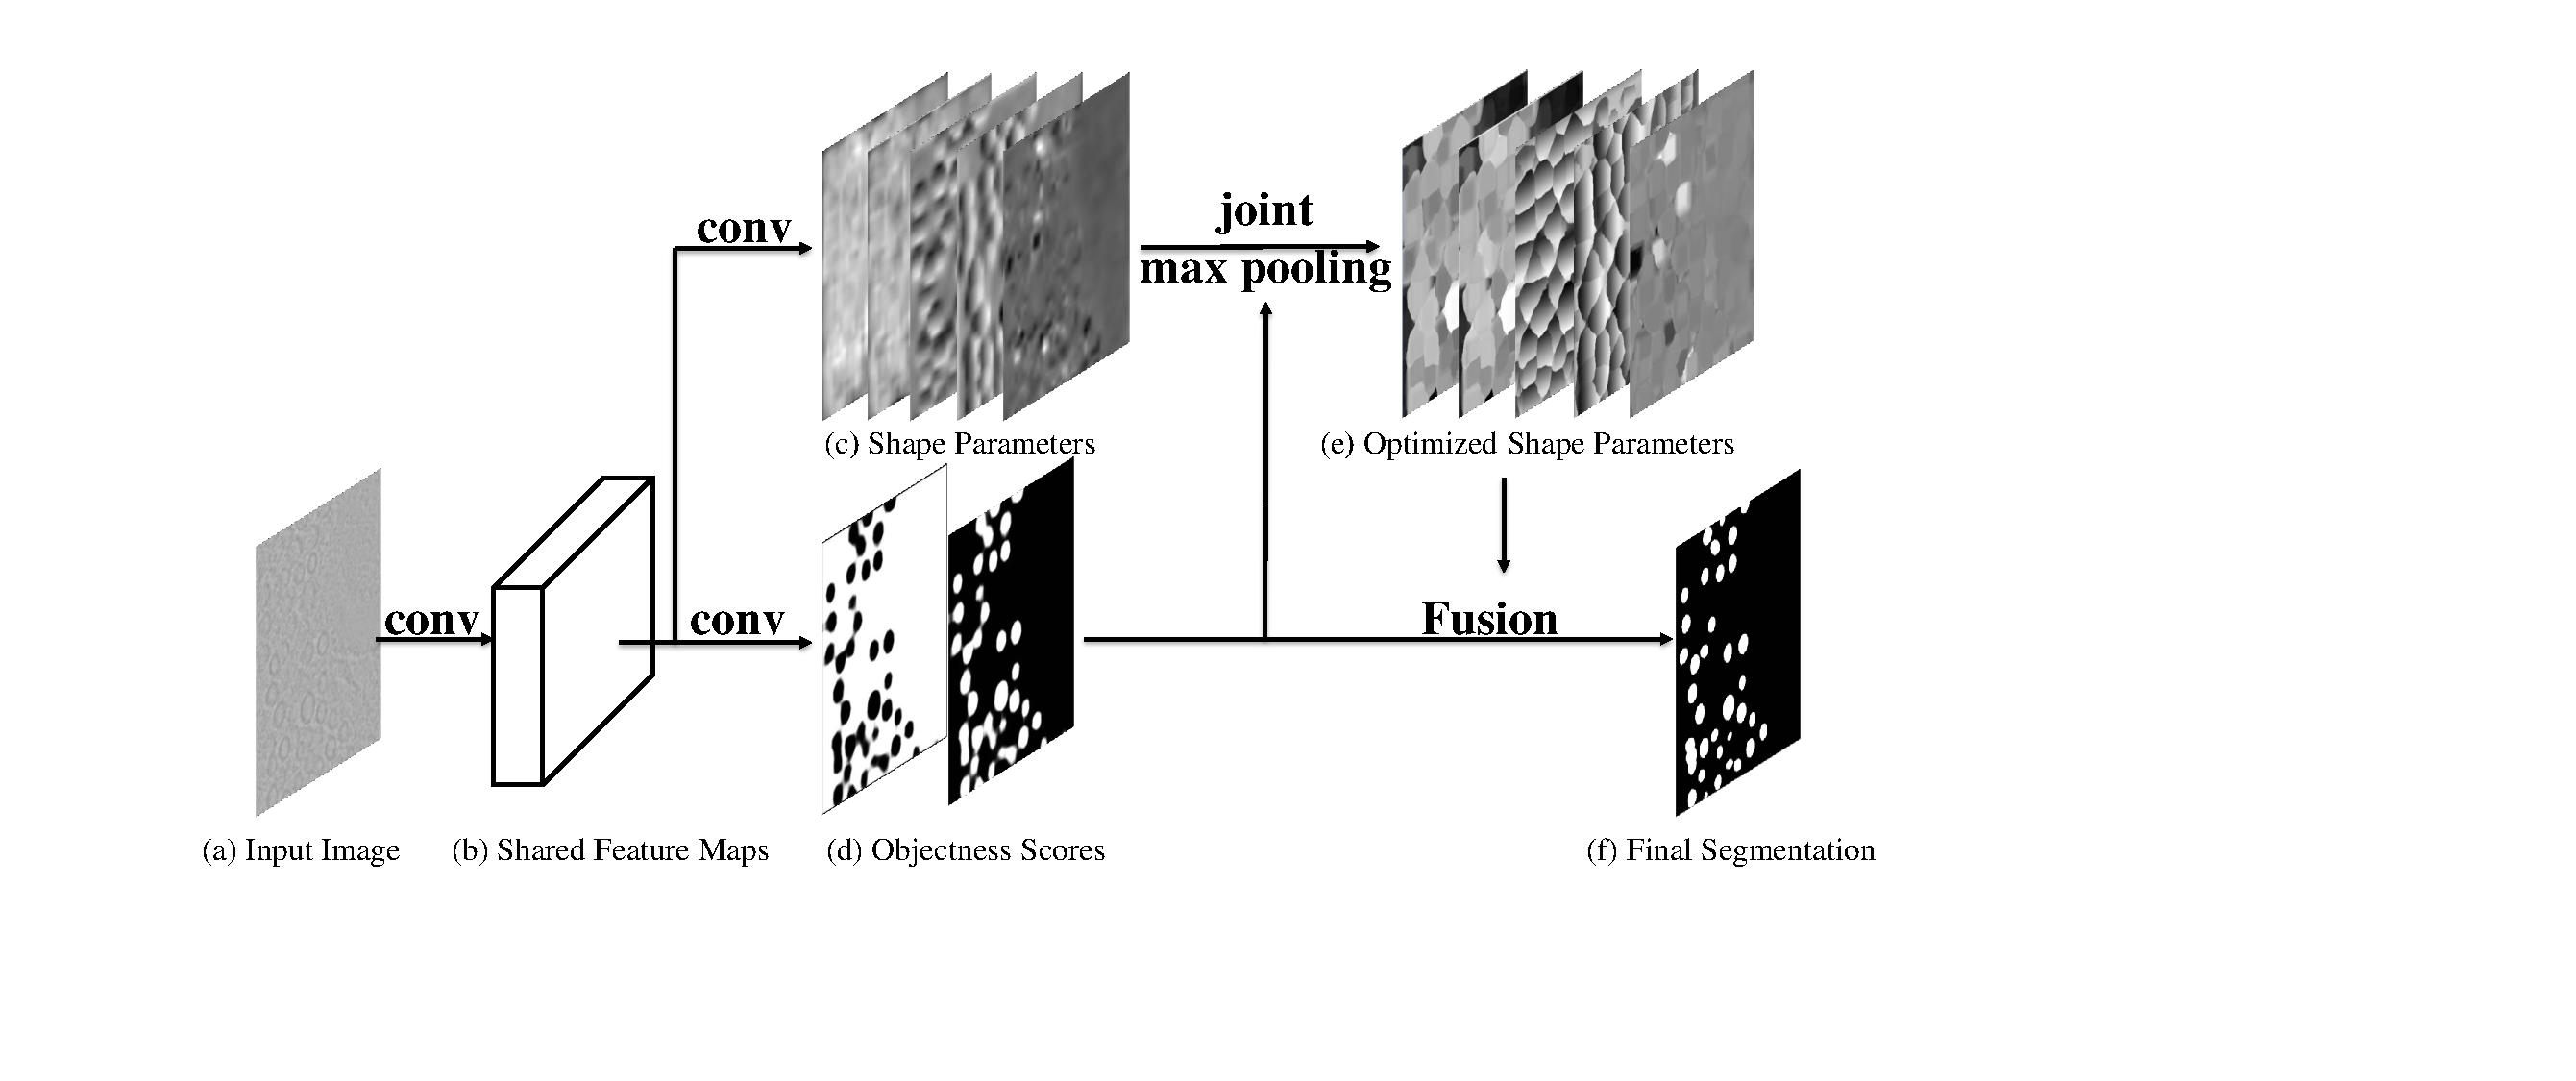
\includegraphics[width=6.3in]{figures/FigSCNN.pdf}
    \end{center}
    \caption{Overview of our proposed scnet. Given an image (a), multi-task neural network simultaneously predict objectness scores (d) and shape parameters of objects (d) using shared feature maps (b).
    Then a joint max pooling is applied to pool (c) with (d) and output new shape parameters (e).
    Finally, segmentation mask (f) is obtained by fusing objectness (d) with the parameterized contour description (e).}
    \label{FigSCNN}
\end{figure*}

Recently, deep neural networks have demonstrated excellent performance in biomedical image segmentation with the use of fully convolutional networks \cite{Dhungel2015,Ronneberger2015,Roth2015,Chen2015,Lieman-Sifry2017,Xu2016,Chen2016b}.
However, as most of these deep networks are based on fully convolutional networks~\cite{Long2015}, the pooling and downsampling layers usually make their localized object boundaries poor and coarse.
To this end, many efforts have been made recently to increase the boundary accuracy.
An U-shaped deep network called U-net~\cite{Ronneberger2015} is proposed for biomedical image segmentation.
By employing the skip connections between contracting and expanding paths, context information can be directly propagated to higher resolution layers for detail preserving.
Several improvements of U-net were proposed soon afterwards.
For example, DeepVentricle~\cite{Lieman-Sifry2017}, which uses the same padding instead of valid padding, has been successfully used for cardiac segmentation.
Recently, DCAN~\cite{Chen2016a} integrates complementary information of objects and contours in a multi-task learning framework to separate the clustered objects into individual ones, which obtains the state of the art performance.
Although these methods achieved promising results in their segmentation tasks, they may fail to achieving satisfying performance in denser and smaller objects with regular shapes, such as synaptic vesicle dataset shown in Figure~\ref{FigImgs}.

In this paper, we propose a first Shape-Constrained neural network (SCNN) to segment dense objects by inherently incorporating prior shape knowledge into network.
Similar with \cite{Chen2016a,Chen2016,Bertasius2016}, we formulate the network as a multi-task learning framework by simultaneously predicting an objectness score map and several auxiliary maps for an input image.
Instead of contour probability as auxiliary, our SCNN learns the parameterized expression of objects shape, which emphasizes more on the overall shape of objects.
Inspired by Region Proposal Network in \cite{Ren2015}, our SCNN simultaneously predicts an objectness score and a set of parameters, formulating the shape of a nearest object, for a pixel.
The complementary information in auxiliary parameters can not only separate the objects into individual ones, but also optimize their shapes.

However since the objects are not always identical, their shape cannot be parameterized uniformly and constrained strictly.
Thus, we select a best representative shape as the soft constraint \bobo{need a better description?} and optimize the predicted shape in a balanced manner between regularization and unconstraint.
In this way, our SCNN not only optimizes the segmented shape of regular objects with prior shape knowledge, but also accommodates seriously deformable shape.


Besides for shape parameters, predicting in boundary of an object is usually harder than that in center, because larger reception field is required by a boundary pixel to explore the complete context of an object.
To this end, we proposed a novel joint max pooling (JMP) to improve the both objectness scores and shape parameters by exploring the intrinsic correlation between them.
Moverover, JMP is designed as a trainable layer, which can be trained end-to-end and easily extended to any multi-task networks.

Overall, the contribution of this paper is three-fold:
\begin{enumerate}
	\item We first effectively incorporate shape constraint into deep neural networks.
	% for biomedical image segmentation.
	\item We propose a novel joint max pooling for benefiting both multi-task outputs.
	\item Our framework is applicable to a series of different tasks such as biomedical image segmentation, scent detection task and achieves the state-of-the-art performance.
\end{enumerate}
